\chapter{Evaluation}

The system has evolved with several user tests along the way.
During the course of the IMPROVE program several features were tested and enhanced.
The shape modeling operations, examine navigation mode
and building creation module were developed later on and were focus of the final user tests.


\section{Intermediate Tests}

% IMPROVE INTRO
Early stages of development of Urban Sketcher were supported by the European Union's
IMPROVE consortium \cite{SITE-IMPROVE}. IMPROVE joined universities, hardware manufacturers
and design studios in the areas of architecture and car design.
Early prototypes of the interface and most of the navigation and reviewing functionalities
were developed during the period of the program. The interface, then called ImmiView,
was used for experimenting large screen display, tablet PC and head-mounted displays on tasks
of architecture design and reviewing sessions.

IMPROVE was beneficial for the large brainstorming sessions which defined several of the concepts
available today on Urban Sketcher, as with the series of User Tests which took place both in
Glasgow Scotland and Lisbon Portugal.
These tests served to get feedback on interface design and the
navigation modes available at the time: first person and compass modes and the multimodal flight mode.


\subsection{Test Environments}

The first Glasgow test occurred between the 16th and the 19th of April 2007 at the Glasgow Caledonian University.
A hand-made screen frame was mounted and one infrared camera calibrated behind the screen.
One regular XVGA projector was used with forward projection.

The Lisbon tests took place between the 11th and 12th of June 2007 and focused on evaluating collaboration tasks.
For these tests the Instituto Superior T�cnico Multimedia Lab was used\cite{LEME}. It has a structure of 4 by 3 projectors
behind a translucent screen. The projection was performed from the back, with 2 infrared cameras mounted on the
projector structure so a bigger portion of the screen to be tracked.

The second Glasgow test occurred between the 16th and 19th of July 2007 at The Lighthouse.
This test was performed on a portable display and a projector with back projection was used along with one infrared camera
for laser tracking.
4 STT system cameras and reflective markers were used for tracking the user's arms.
One Microsoft ZX-6000 wireless headset microphone was used to get the user's voice and the Microsoft Speech API 5.1
American English version performed speech recognition to identify a set of commands issued by the user.

\begin{figure}[ht]
	\centering
		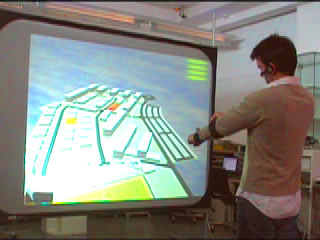
\includegraphics[scale=0.75]{gfx/don.png}
	\caption{User performing multimodal flight during the Lighthouse test}
	\label{fig:don}
\end{figure}


\subsection{Results}

The test at Caledonian provided feedback about the navigation first person and compass navigation modes.
The layout of the first person mode was changed -- its gates layout used to mimic the 3 axis for movement and had
rotation gates in between. These were changed to the cleaner design we have today.
The compass mode was enthusiastically adopted. It used to feature additional gates to move up/down and zoom compass view.
These gates were dropped to obtain a simpler design.

The Lisbon tests proved the system could handle collaborative design and review tasks.
\TODO{MORE?}

The Lighthouse test focused on testing the flight navigation mode. One user had to wear 4 velcro fabric strips
with reflective markers and a wireless microphone. A 3 by 3 meters area in front of the screen was tracked by
motion tracking cameras.
\TODO{...}




\section{Final Tests}

The final tests were conducted several months later, with the system fully centered on the Urban Sketcher
objectives and features. The most notorious features were tested in a series of small tasks: 2 for navigation,
2 for shape modeling and one for building manipulation. To have reference data from which to compare to,
one of the analyzed systems on the Related Work section, Google SketchUp, was also used on the test.
Both the navigation and shape modeling tasks were performed on SketchUp -- building manipulation isn't supported by the system.

It is important to highlight that Google SketchUp is a commercial product with several years of development and
is based on familiar interface concepts and tested on a regular computer screen with keyboard and mouse input.
On the other hand Urban Sketcher tests are to be performed on a large screen display using a laser pointer
and an \emph{ad hoc} laser tracking system, with a set of novel interface concepts.


\subsection{Test Environment}

The final tests took place on the Instituto Superior T�cnico Multimedia Lab between the 28th of June and 1st of July 2008.
The tests were performed with the same environment as the Lisbon IMPROVE test described above -- a large display screen
of 4 by 3 projectors on a translucent screen. The laser tracking system was calibrated to get only laser information
from about 1/3 of the screen area. During the 4 days period 16 users performed a series of tests described below.
The distributed documents for task performance and questionnaires can be found on appendix \ref{finalTests}.
94\% of the users had college degrees, 31\% were women and the average user age was 37 years old.

User tests were performed individually and took between 60 and 90 minutes.
First a preliminary questionnaire composed of 5 close-ended scaled questions was handed and filled, to assert the past experience
of users on relevant topics.
Then the purpose of the project was presented along with a tutorial of Urban Sketcher's features and how to use them.
After a small hands-on period the tasks were given to the user to perform on the Urban Sketcher system.
Then a tutorial was given of the Google SketchUp program, focused on the features necessary to perform the tasks.
Alter a small hands-on period the navigation and modeling tasks were performed on the Google SketchUp system.
To finalize the test, the final questionnaire was handed and filled. It was composed of 13 close-ended scaled questions
and 5 open-ended questions, the former to obtain feedback regarding the Urban Sketcher system and the latter
focused on comparing the two systems.


\TODO{MULTIMEDIA WALL DIAGRAM, TRACKED SCREEN AREA}

\subsection{Results}

During the tests task completion time was measured in minutes and both user errors and system unexpected events were
logged. On table \ref{table-times} the summary of times for completing all the tasks is listed.
Chart \ref{graph-comparison} depicts average times for completing the tasks on both systems.


\begin{table}[!ht]
	\centering
		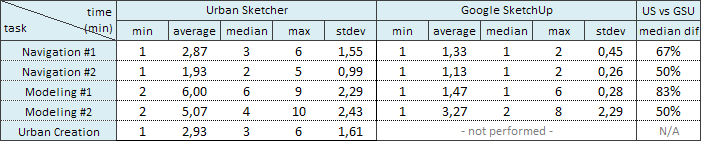
\includegraphics[scale=0.6]{gfx/eval/table-times.png}
	\caption{Task completion times on Urban Sketcher and Google SketchUp}
	\label{table-times}
\end{table}


\begin{figure}[!ht]
	\centering
		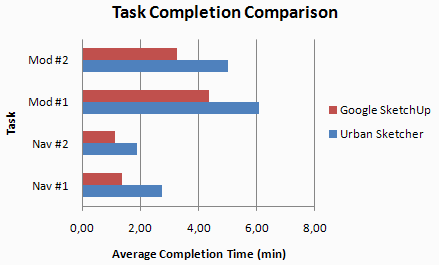
\includegraphics[scale=0.6]{gfx/eval/graph-comparison.png}
	\caption{Bar chart comparing task completion times on both systems}
	\label{graph-comparison}
\end{figure}


The questionnaires feature a total of 18 close-ended scaled questions. These had to be graded from 1 to 6, with
1 meaning complete disagreement to/infrequent statement and 6 completely agree/very frequent. Out of these questions,
the first 5 tested the users past experience in relevant topics and the remaining 13 got feedback on using Urban Sketcher.
Additionally, 5 open-ended questions were given at the end, focusing on the comparison of both systems.

The translated questions and their results are listed on tables \ref{table-questions18} and \ref{table-questions5}.
To aid in the interpretation of these results, charts \ref{graph-quantified} and \ref{graph-pies} were respectively created.

\begin{table}[!ht]
	\centering
		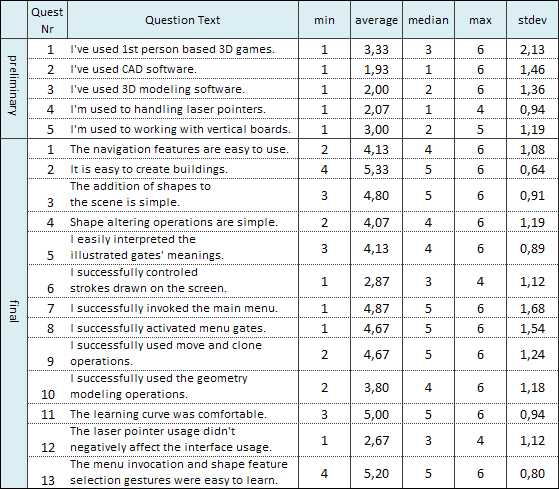
\includegraphics[scale=0.6]{gfx/eval/table-questions18.png}
	\caption{Preliminary and Final Questionnaire close-ended questions and results}
	\label{table-questions18}
\end{table}


\begin{table}[!ht]
	\centering
		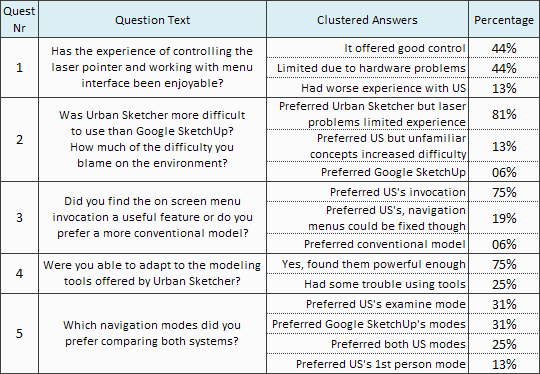
\includegraphics[scale=0.6]{gfx/eval/table-questions5.png}
		\caption{Final Questionnaire open-ended questions and clustered answers}
	\label{table-questions5}
\end{table}


\begin{figure}[!ht]
	\centering
		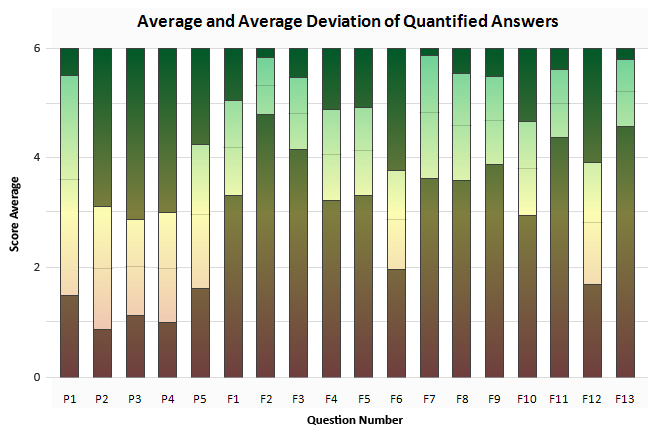
\includegraphics[scale=0.6]{gfx/eval/graph-quantified.png}
		\caption{Chart illustrative of close-ended answers, average value and uncertainty}
	\label{graph-quantified}
\end{figure}



\begin{figure}[!ht]
	\centering
		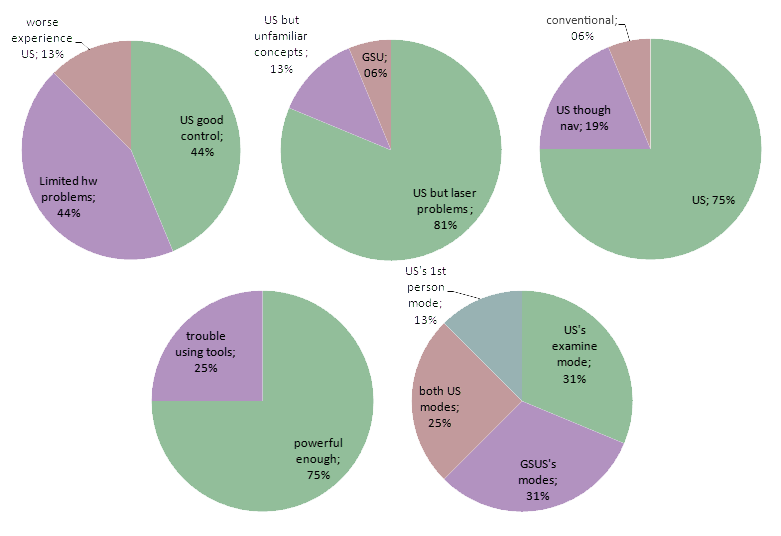
\includegraphics[scale=0.5]{gfx/eval/graph-pies.png}
		\caption{Pie charts featuring the clustered open-ended answers}
	\label{graph-pies}
\end{figure}


\subsection{Discussion}

% US vs GSO - tempos, diferen�as, issues

\subsubsection{Task Performance and Issues}

When looking at the average time it took users to complete the tasks,
Urban Sketcher results have taken between 28\% and 50\% more time than Google SketchUp.
This difference is surprisingly small given that users performed Urban Sketcher tasks standing up,
using a novel user interface and handling a laser pointer on a limited tracking area.

The navigation tasks were the first to perform, with users getting used to the interface.
Some undesired context menus were invoked at these first tasks, probably due to users drawing too fast,
which segments the real strokes into small segments, misleading the system into recognizing these context menu invocations.

It was on the modeling tasks that those differences were less notable.
This can be inputed to the carefully crafted modeling operations and their menus.
Some users took more time grasping the concept of stroke-long operations and their requirement to
keep the stroke active after triggering the operation to set its direction and length.
The main menu stroke gesture (a closed triangle) had worse recognition success on these operations.
This might have to do with users performing more context menu invocations and temporarily forgetting the correct
gesture to invoke the main menu or drawing triangles more roughly.

The building creation task was performed very smoothly in regard to its complexity.
Only a small set of individual problems occurred and users felt satisfied with the easy at
which they instanced buildings and assets.


\subsubsection{Close-ended Answers Analysis}

% perguntas fechadas - 1o mais certas, depois mais favor�veis
The familiarity of users with 3D software and CAD is low and the usage of 3D first person games is disparate.
Few users were used to handling laser pointers and some of them used vertical boards occasionally
-- this might be explained by the presence of 2 teachers on the user test.

Users found navigation, creation of buildings and shape creation and modeling fairly easy.
The illustrated gates were given a good recognition ratio and their activation was successful.
Menu invocation and shape feature selection were easy to learn.
Both the move and clone operations were credited as functional and the learning curve classified comfortable.

Users diverged the most when asked about the success at which they controlled their strokes.
This problem can be credited to the laser tracking limitations on both tracked screen area and slow capturing frequency.
These originated visual deviations between real stroke and its interpretation, especially notable near the tracking boundaries.
Due to the slow capturing frequency, strokes had to be drawn slowly, otherwise they'd get segmented.
This problem was emphasized when performing apply-to-scene operations such as re-centering the examine center of interest or instancing new shapes which required continuity of stroke.


\subsubsection{Open-ended Answers Analysis}

Most users held the laser tracking facilities responsible for some dissatisfaction and slowness in performing the tasks
when comparing with Google SketchUp (81\% of the users).
13\% of the users felt the novel interface unfamiliar therefore harder to master for a novice user while only 6\% elected
Google SketchUp as the best interface.
94\% of the users enjoyed the capacity of invoking menus as needed -- of these, 13\% pointed out that the navigation menu
could be fixed to the screen due to its constant usage, though this screen allocation problem was result solely of the
limited tracked area of screen -- if all screen was being tracked the menu could have remained there the whole time.
Out of all the users, only 25\% state having trouble with the modeling tools. This is satisfactory since many users
have shown low confidence at first when asked to perform the modeling tasks, ending up completing them with success and
reasserting their beliefs regarding such tasks. Several users felt this interface could be very effective on several domains
for controlling large screen displays.

It was shown that a stroke-based interface is capable of offering a set of complex actions and navigation modes to novice users
with them successfully performing tasks in reasonable time frames. Most users identified the laser tracking input as an obstacle
to an even better experience. This is a technical limitation which doesn't invalidate the application of these concepts and
interface with other technologies such as large multi touch surfaces.


% perguntas abertas - compara��o?!